\chapter{Comparison with state-of-the-art benchmarks and Challenges faced}

\begin{table}[!htb]
\centering
\captionsetup{
justification = centering
}
\caption{Comparison with state-of-the-art benchmarks}
\begin{tabular}{|c|c|c|c|}
\hline
\textbf{Topology} & \textbf{\begin{tabular}[c]{@{}c@{}}FPGA \\ execution time\end{tabular}} & \textbf{\begin{tabular}[c]{@{}c@{}}OpenVINO CPU  \\ execution time\end{tabular}} & \textbf{\begin{tabular}[c]{@{}c@{}}Microsoft \\ Brainwave\end{tabular}} \\ \hline
GoogLeNet & 1.18 sec  & 8.79 ms & -\\ \hline
ResNet–50 & 10.77 sec & 19.42 ms & 4 ms \\ \hline
\end{tabular}
\label{tab:Comp_benchmarks}

\end{table}
Table \ref{tab:Comp_benchmarks} shows the comparison of execution times of different topologies on different devices and on a deeplearning platform, Microsoft Brainwave. OpenVINO CPU plugin was executed on cc-frontend with 16 CPUs, 4 cores in each socket running at 3.7 GHz,  OpenVINO FPGA plugin was executed on multiple Intel Stratix 10 FPGAs in the noctua infrastructure and Microsoft Brainwave executes the CNN topologies on one Stratix 10 FPGA.

For GoogLeNet topology, execution time on OpenVINO CPU plugin was 8.79ms and on OpenVINO FPGA plugin was 1.18s. Microsoft Brainwave did not support this topology. Whereas for ResNet topology, execution time on OpenVINO CPU plugin was 19.42ms, on OpenVINO FPGA plugin was 10.77s and Microsoft Brainwave took execution time of 4ms on 1 FPGA.

 We observed that the difference in execution time of the topologies is very vast when compared FPGA plugin and CPU plugin. Hence, we examined deep to find out the probable causes for this difference. 

%End of Chapter
\section{Causes of sub-optimal results} 
\label{sec:challenges}

\begin{enumerate}

\item\textbf{Low level parallelism: } The OpenVINO CPU plugin is highly optimised and highly parallel in the sense it executes thousands of instructions parallely on the CPU running at the frequency of GHz. On the other hand, we have been able to execute approx 150 instructions parallely at the frequency of MHz. Hence there is a significant due to this reason.
\item\textbf{FPGAs idle time: }
The GoogleNet and ResNet CNN models have a sequential architecture. Since the whole network is too big to fit in one FPGA, we divide the structure into several small sub-structure and then execute them on several FPGA. Due to sequential architecture, the next sub-structure is dependent on the previous sub-structure, hence the next FPGA has to wait till the previous FPGA completes the execution.
Parallel execution of FPGA is required to solve this which can be done with the help of channels to handle the data between the FPGAs. Also, Batch processing could help in increasing the utilisation and efficiency of FPGAs
\begin{figure}[h!]
  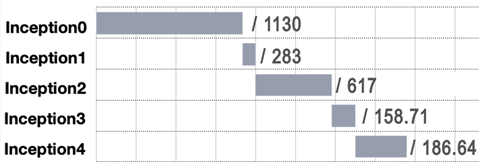
\includegraphics[width=\textwidth,height=\textheight,keepaspectratio]{img/fpga_idle.png}
  \caption{Most of the time FPGA is idle }
  \label{fig:FPGA_idle_time}
\end{figure}
\item\textbf{Accumulated Data: }
The kernel design that we have used in GoogleNet hybrid design makes use of internal and external IO channels. These kernels work on accumulated data, i.e., the kernel starts processing after only it has received the complete set of data from the channels. Hence the kernels here are idle till they don’t receive the whole data. One way to solve this issue is to use a Streaming design. Streaming design have data pipelined in its architecture thereby eradicating the idle time of the kernels
\begin{figure}[h!]
  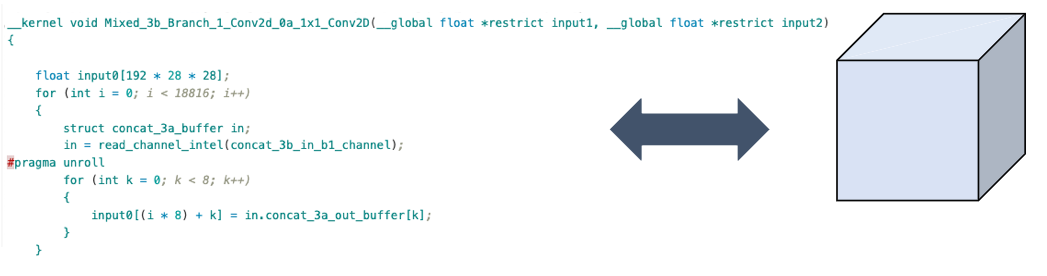
\includegraphics[width=\textwidth,height=\textheight,keepaspectratio]{img/accumulated_data.png}
  \caption{Data accumulating but not immediately processing }
  \label{fig:Data_accumulation}
\end{figure}
\item\textbf{Trade-off between Factors: }
While synthesizing kernels several factors play a keen role in the synthesis. High resource utilisation has a direct effect on synthesis time, i.e., high resource utilisation could result in high synthesis time. On the other hand, design of the kernels has a significant impact on the Fmax of the kernels. There could be a scenario where a particular design could yield a higher Fmax but requires more resource hence it will increase the synthesis time of the kernels. Therefore it is hard to find a trade-off between these factors and hit the perfect spot where all these factors are balanced.
\item\textbf{Lack of Experience: }
Since the whole team is new to the kernel development and FPGA infrastructure, we are in a continuous state of self-development by venturing out several ideas and concepts in the kernel development and will gain experience over time.

\end{enumerate}


\section{Quantization Issues }
One of the initial goals listed in the project plan was to perform Quantization. Quantization involves low precision math and hence can positively impact various performance metrics of our project. This was the motivation behind choosing this subgoal. Among various approaches available to achieve this, after discussion and research, we decided to implement Post Training Quantization which is supported by both TVM and OpenVINO. The Calibration Tool present in the latest release of OpenVINO performs post-training quantization of the CNN model to int8 before the model’s IR is passed on to the inference engine. This task is less time consuming and less complex as we don’t have to retrain the model using quantized weights. Also, we were able to generate kernels using TVM’s quantize function. 

Although most of the aspects seemed to fall into place, we came across two potential risks that hindered us in achieving this goal. 
		
\begin{itemize}
\item The version of OpenVINO used in the project (2018 R5) only supports FP16 or FP32 operations. The Post Training Quantization discussed previously is available in the latest version (2019 R1). This implied that we should migrate our project 2018 R5 version to the new one. During that time of the project, many branches of the repository were simultaneously under development and it made migration difficult. 
\item To support migration to a new version of OpenVINO, we also may be required to make modifications to the existing FPGA plugin and again, this would involve understanding the changes, impact analysis and development. Due to the limited amount of time available, even this affected our decision to stop pursuing this goal.
\end{itemize}
